\documentclass{article} %[letterpaper]
% https://github.com/Jordy-VL/latex-templates/blob/master/papers/preamble/preamble.tex

% FONTS
\usepackage{times}
\usepackage{helvet}
\usepackage{courier}
\usepackage[utf8]{inputenc} % allow utf-8 input
\usepackage[T1]{fontenc}    % use 8-bit T1 fonts
\usepackage{amsfonts}       % blackboard math symbols
\usepackage{nicefrac}       % compact symbols for 1/2, etc.
\usepackage{microtype}      % microtypography

% IMAGES & TABLES
\usepackage{graphicx}
\usepackage{booktabs} % for professional tables
\graphicspath{ {images/} }
\usepackage{enumitem}
\usepackage{array,amsmath}
\usepackage{amsthm,amssymb}
\usepackage{bbold} % for \mathbb

\usepackage{preamble/custom-conf}

%everything following here changes defaults
\usepackage[font=footnotesize,skip=5pt, belowskip=-10pt,labelfont=it]{caption}
\usepackage{subcaption}

% # APPENDIX
\renewcommand \thepart{}
\renewcommand \partname{}


%%%%%%%%%%%%%%%%%%%%%%%%%%%%%%%%%%%%%%%%%%%%%%%%%%%%%%%%%%%%%%%%%%%%%%%%%%
%                               PROOF, THEOREM, and FRIENDS
%%%%%%%%%%%%%%%%%%%%%%%%%%%%%%%%%%%%%%%%%%%%%%%%%%%%%%%%%%%%%%%%%%%%%%%%%%%

\newcommand{\BlackBox}{\rule{1.5ex}{1.5ex}}  % end of proof
%\newenvironment{proof}{\par\noindent{\bf Proof\ }}{\hfill\BlackBox\\[2mm]}
\newenvironment{derivation}{\par\noindent{\bf Derivation\ }}{\hfill}
\newtheorem{example}{Example} 
\newtheorem{problem}{Problem} 
\newtheorem{theorem}{Theorem}
\newtheorem{lemma}[theorem]{Lemma} 
\newtheorem{proposition}{Proposition}  %[theorem]
\newtheorem{remark}{Remark}
\newtheorem{corollary}{Corollary}
\newtheorem{definition}{Definition}
\newtheorem{conjecture}[theorem]{Conjecture}
\newtheorem{axiom}[theorem]{Axiom}
%https://tex.stackexchange.com/questions/109843/cleveref-and-named-theorems

% For pseudo algorithms
\usepackage[linesnumbered,ruled,vlined]{algorithm2e}
\SetKwComment{Comment}{$\triangleright$\ }{}
\newcommand\mycommfont[1]{\tiny\ttfamily\textcolor{blue}{#1}}
\SetCommentSty{mycommfont}

% Custom math shortcuts
\newcommand{\argmin}{\arg\!\min}
\newcommand{\argmax}{\arg\!\max}
%\DeclareMathOperator*{\argmax}{argmax} % thin space, limits underneath in displays
\newcommand*{\defeq}{\stackrel{\text{def}}{=}}
\DeclareMathOperator*{\CE}{\operatorname{CE}}
\DeclareMathOperator*{\SCE}{\operatorname{SCE}}
\DeclareMathOperator{\Prob}{\mathbb{P}}
\DeclareMathOperator{\Exp}{\mathbb{E}}
\newcommand{\ubar}[1]{\text{\b{$#1$}}}

% # Tabular elements
\usepackage{tabularx}
\usepackage{arydshln}

\setlength{\dashlinedash}{0.2pt}
\setlength{\dashlinegap}{4.5pt}
\setlength{\arrayrulewidth}{0.2pt}
%new column types: H to hide, Z to hide and remove padding last col
\newcolumntype{H}{>{\setbox0=\hbox\bgroup}c<{\egroup}@{}}
\newcolumntype{Z}{>{\setbox0=\hbox\bgroup}c<{\egroup}@{\hspace*{-\tabcolsep}}}

% # COUNTERS

\renewcommand{\labelenumi}{\color{black!67}{\arabic{enumi}.}}
\renewcommand{\labelenumii}{{\color{black!67}(\alph{enumii})}}
\renewcommand{\labelitemi}{{\color{black!67}\textbullet}}

% # CUSTOM colors

\definecolor{shadecolor}{gray}{0.9}
\newcommand{\red}[1]{\textcolor{BrickRed}{#1}}
\newcommand{\orange}[1]{\textcolor{BurntOrange}{#1}}
\newcommand{\green}[1]{\textcolor{OliveGreen}{#1}}
\newcommand{\blue}[1]{\textcolor{MidnightBlue}{#1}}
\newcommand{\sky}[1]{\textcolor{SkyBlue}{#1}}
\newcommand{\gray}[1]{\textcolor{black!60}{#1}}
\usepackage{xcolor,colortbl}

% # References and LINKS

\usepackage[nameinlink,capitalise]{cleveref}
%\crefname{section}{§}{§§}
%\Crefname{section}{§}{§§}
\creflabelformat{equation}{#2\textup{#1}#3}  % <- remove parenthesis from equations

% # TODO package for commenting (to not mess up the whole text)
%Todos package
\usepackage{xargs}  % Use more than one optional parameter in new command
\usepackage[colorinlistoftodos,prependcaption,textsize=tiny]{todonotes}
\definecolor{OliveGreen}{cmyk}{0.64,0,0.95,0.40}
\definecolor{ForestGreen}{RGB}{34,139,34}
\colorlet{darkgreen}{green!60!black!80!}
\colorlet{darkorange}{orange!60!black!80!}
\colorlet{purple}{red!80!green!20!blue!60!}
\definecolor{alizarin}{rgb}{0.82, 0.1, 0.26}
\definecolor{cadmiumgreen}{rgb}{0.0, 0.42, 0.24}


% # REVIEWING

%\setlength{\marginparwidth}{4.5cm}
\newcommandx{\unsure}[2][1=]{\todo[linecolor=red,backgroundcolor=red!25,bordercolor=red,#1]{#2}}
\newcommandx{\change}[2][1=]{\todo[linecolor=blue,backgroundcolor=blue!25,bordercolor=blue,#1]{#2}}
\newcommandx{\info}[2][1=]{\todo[linecolor=OliveGreen,backgroundcolor=OliveGreen!25,bordercolor=OliveGreen,#1]{#2}}
\newcommandx{\improvement}[2][1=]{\todo[linecolor=ForestGreen,backgroundcolor=ForestGreen!25,bordercolor=ForestGreen,#1]{#2}}

\newcommandx{\draft}[2][1=]{\todo[linecolor=ForestGreen,backgroundcolor=ForestGreen!25,bordercolor=ForestGreen,inline,caption={},#1]{\small #2}}
\newcommandx{\draftp}[2][1=]{\todo[linecolor=ForestGreen,backgroundcolor=ForestGreen!25,bordercolor=ForestGreen,inline,#1,noprepend,caption={}]{\small #2}}

\newcommandx{\dcomm}[2][1=]{\todo[linecolor=ForestGreen,backgroundcolor=darkorange!25,bordercolor=ForestGreen,#1]{#2}}
%\newcommandx{\dcomm}[2][1=]{}
%disable comments

\newcommandx{\exactcopy}[2][1=]{\todo[linecolor=darkorange,backgroundcolor=darkorange!25,bordercolor=darkorange!50,inline,#1,noprepend,caption={}]{\small #2}}

\newcommandx{\summarize}[2][1=]{\todo[linecolor=blue,backgroundcolor=blue!25,bordercolor=blue,#1]{\normalsize #2}}

\newcommand{\rev}[1]{\textcolor{purple}{#1}}
%% Two commands to disable for multiple views
%\newcommand{\rev}[1]{#1}
%\newcommandx{\thiswillnotshow}[2][1=]{\todo[disable,#1]{#2}}
\newcommand{\fix}{\marginpar{FIX}}
\newcommand{\new}{\marginpar{NEW}}


% # VISUALS on MATH
\newcommand{\highlight}[1]{\mathpalette\highlightwithstyle{#1}}
\newcommand{\highlightwithstyle}[2]{\colorbox{red!50}{$#1#2$}}

\usepackage{mathtools}% superior to amsmath
\usepackage{tikz}
\makeatletter
\newcommand\mathcircled[1]{%
	\mathpalette\@mathcircled{#1}%
}
\newcommand\@mathcircled[2]{%
	\tikz[baseline=(math.base)] \node[draw,circle,inner sep=1pt] (math) {$\m@th#1#2$};%
}
\makeatother

\usepackage{circledsteps}
%\usepackage{pstricks}

  
% lists 
\usepackage{enumitem,amssymb}
\newlist{todolist}{itemize}{2}
\setlist[todolist]{label=$\square$}

\usepackage{pifont}
\newcommand{\cmark}{\ding{51}}%
\newcommand{\xmark}{\ding{55}}%
\newcommand{\done}{\rlap{$\square$}{\raisebox{2pt}{\large\hspace{1pt}\cmark}}%
	\hspace{-2.5pt}}
\newcommand{\wontfix}{\rlap{$\square$}{\large\hspace{1pt}\xmark}}


\usepackage[preprint]{stys/neurips_2021}
\usepackage{natbib}

\makeatletter
\def\blfootnote{\gdef\@thefnmark{}\@footnotetext}
\makeatother

\title{Charlie is All You Need: an Empirical Study} 

\author{Jordy Van Landeghem$^{*}$ \\
  Papa \\
  Dept. of Computer Science\\
  \textit{LIIR}, KU Leuven, Belgium \\
  Contract.fit, Brussels, Belgium\\
  \texttt{first.lastname@cs.kuleuven.be} \\\And
   Marijke Leysen$^{*}$ \\
   Mama \\
  De Kleine Berg \\
  \textit{Kinderopvang}, Boechout, Belgium \\
  \texttt{marijkeleysen@hotmail.be} \\
  }

\begin{document}

\setcounter{section}{0}
\blfootnote{*: Joint first-authors.}

\maketitle

\begin{abstract}

Having a child is a blessing as well as a huge commitment. In this joint empirical study, the co-authors have managed to create a new lifeform, denoted as project \textbf{Charlie} (working title). This paper reports on the progress made throughout project Charlie, from the first discovery of pregnancy to the monthly check-ups and finally the birth of our baby.
The methodology is by no means new, so we differentiate by the depth of our analysis, offering both qualitative and quantitative results.
Thus far, we cannot make any concluding statements, besides that our baby is healthy and that the due date is calculated for \textit{November 9, 2022}.

\end{abstract}

\section{Introduction}%~\ref{sec:intro}
The motivation for project Charlie stems from the genuine love between two humans who have been in a steady relationship for almost 4 years. The origin point was the "Donkfeesten" in Lier, where a famous local cover band has enticed the authors to start a not-so professional relationship.\\
We will assume that the reader has sufficient background on what happened between the start of the co-authors' relationship and continuing up until the discovery of the onset of pregnancy.

On the 7th of March 2022, our world was shocked by learning that Marijke's tummy aches were not caused due to some gastrointestinal parasite, but rather the result of ovulation, followed by fertilization \citep{familiari2006ultrastructural}. From a blood test, we gathered that a certain hormone, human chorionic gonadotropin (hCG) \citep{nwabuobi2017hcg}, was very present with a value of \texttt{5487}. The key provided by the medical laboratory pointed to \textit{Amenorrhea} \citep{practice2004current}, absence of menstruation, of at least 5 weeks.
A phone call to my trusted, general practitioner, Dr. Neutjens, confirmed that we were indeed pregnant. 

At this stage, there was a \textit{zygote} developing within Marijke and we made practical arrangements with a gynecologist for the first, visual \textit{existence proof} of Charlie at week 7.
Below, we illustrate the ultrasound at week 7 and week 12 to compare the evolution from embryo to fetus.    

\begin{figure}[h]
    \centering
    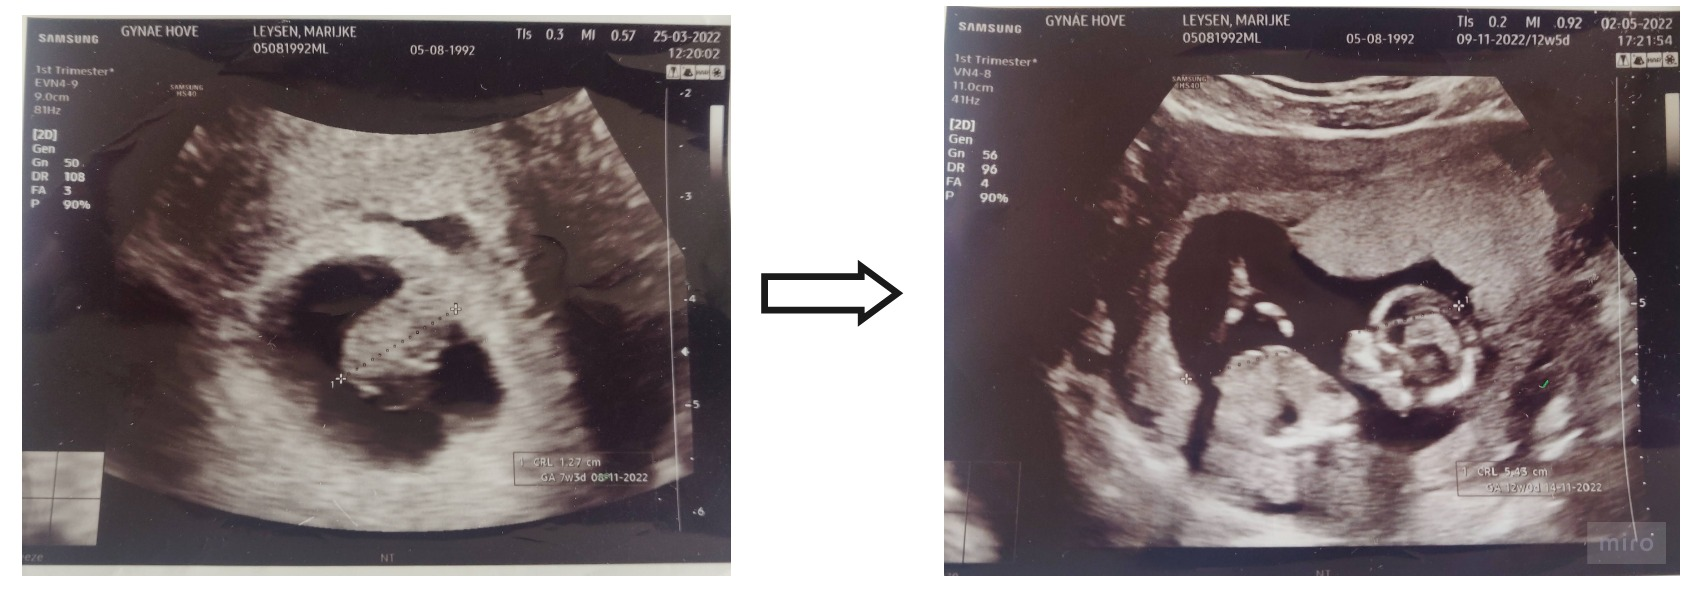
\includegraphics[width=0.5\linewidth]{./images/Charlie-progress.jpg} 
    \caption{Left: 7-week ultrasound scan which shows the embryonic state (week 3-8). 
    Right: 12-week ultrasound scan which shows the fetal state (week 9-onwards).}
    \label{fig:progress}
\end{figure}

Today \today, we are in week 14 and we will definitely keep documenting the ongoing progress of Charlie.

%, that one should only undertake when they are mentally, emotionally and financially ready.
%\begin{figure}
%    %\centering
%    \includegraphics[width=0.5\linewidth]{} 
%    \caption{Graphical representation of a linear-chain CRF. Each of the nodes of the output sequence $y$ depend on the complete input $x$.}
%    \label{fig:linearchaincrf}
%\end{figure}

\bibliography{main.bib}
\bibliographystyle{stys/neurips_2021}

\end{document}

Measuring     
Methods
Conclusions
